\documentclass{article}
\usepackage{titlesec}
\usepackage{lipsum}
\usepackage{hyperref}
\usepackage{graphicx}
\usepackage{appendix}
\usepackage[left=1 in,right=1 in,top=1 in,bottom=1 in]{geometry}

% Remove the red boxes around links
\hypersetup{
    colorlinks=true,
    linkcolor=black,
    citecolor=green,
    urlcolor=blue
}

\titleformat{\section}[hang]{\normalfont\scshape\Large\bfseries}{\thesection}{1em}{}
\titleformat{\subsection}[hang]{\normalfont\scshape\large\bfseries}{\thesubsection}{1em}{}
\titleformat{\subsubsection}[hang]{\normalfont\scshape\normalsize\bfseries}{\thesubsubsection}{1em}{}

\begin{document}

% Title Page
\begin{titlepage}
    \centering
    
\includegraphics[width=0.8\textwidth]{image.jpeg}\par % Adjust the width as needed
     \vspace{2cm}
    {\scshape\Large SOEN 6481: TAS REPORT \par}
    \vspace{1.5cm}
    {\scshape\Huge Topic 58: How should I manage adoption of new technologies or processes in my projects?\par}
    \vspace{1.5cm}
    {\large Advisor: Professor Pankaj Kamthan\par}
    \vspace{1.5cm}
    {\large By: Konark Shah (Student ID: 40232277)\par}
    \vspace{1cm}
    {\large \today\par}
\end{titlepage}

\tableofcontents

\newpage

\section{Abstract}
\lipsum[1]

\section{Introduction}
In today's fast-changing tech landscape, it's crucial for companies to keep up with the competition by adopting and integrating new technologies into their existing products. Making the right decisions in this process is complex and can make or break a new product. To navigate this terrain successfully, one must consider a range of factors, including the nature of the ongoing project, the team's experience and skill set, communication strategies with stakeholders, and the pivotal step of securing approval from top management. This thesis seeks to unravel the complexities surrounding this crucial decision-making process, offering insights into the managerial intricacies involved in the successful adoption of new technologies or processes within projects.


\subsection{Motivation}
This thesis is motivated by a keen interest in unraveling the complexities of adopting new technology and procedures. Recognizing that understanding this complexity is not just beneficial but essential for successful project navigation, the thesis aims to shed light on practical approaches for managing the adoption of new technologies. It aspires to offer valuable insights for project managers, helping them strike a delicate balance between innovation and seamless project execution.

\subsection{Problem Statement}
The fundamental issue addressed in this paper is the successful management of new technology or process adoption within project environments. The complexity stems from the opposition encountered during major changes, the uncertainties around cost and benefit projections, and the requirement for a proactive strategy to obtain buy-in from contributors and stakeholders. Prudent decision-making in this setting necessitates a thorough awareness of the issues at hand, as well as the creation of appropriate mitigation methods.

\subsection{Research Questions}
\begin{enumerate}
    \item[Q1:] How can project leaders efficiently assess the costs and benefits of adopting new technologies or processes, including estimating the consequences of maintaining the status quo?
    
    \item[Q2:] What strategies help project leaders plan for team skills, knowledge, and resistance when implementing major changes in a project?
    
    \item[Q3:] What elements make a business case persuasive, and how can project leaders tailor communication to align with the interests of stakeholders?
    
    \item[Q4:] How do project managers manage risks and uncertainties in adopting new technologies or processes, and what role does contingency planning play in successful implementation?
\end{enumerate}


---
\subsection{Critical Thinking}

The research questions mark a pivotal stage in investigating the challenges of implementing new technology or processes in projects. Each question represents careful thought on project dynamics, organizational context, and the complexity associated with technological integration.

\subsubsection*{Q1: Efficient Assessment of Costs and Benefits}

For the first question (Q1), it focuses on the pragmatic aspects of project leadership. It aims to understand how project leaders can efficiently assess costs and benefits, balancing the existing state against potential advancements.

\subsubsection*{Q2: Strategies for Planning in the Face of Change}

The second question (Q2) addresses the necessity for strategic planning in implementing major changes. This inquiry seeks strategies for project leaders to navigate challenges related to team skills, knowledge, and resistance during technological integration.

\subsubsection*{Q3: Persuasive Business Cases and Stakeholder Alignment}

The third question (Q3) stems from recognizing communication’s role in technology adoption. We explore the elements that make a business case persuasive, emphasizing stakeholder alignment as crucial for successful integration.

\subsubsection*{Q4: Risk Management and Contingency Planning}

The fourth question (Q4) underscores our commitment to addressing uncertainties tied to technological adoption. The aim is to uncover how project managers can proactively manage risks, emphasizing the role of contingency planning in ensuring successful implementation.
\newline

\noindent In formulating these questions, the critical thinking process delved into the nature of project changes, the team's experience, and the broader implications of technological integration. Each question strategically explores the "how" and "why" of effective project management practices amid technological evolution. The subsequent section outlines specific objectives, providing a road map.



\subsection{Objectives}

The objectives of this investigation are to:

\begin{itemize}
  \item Evaluate the impact of project nature and team experience on technology and process adoption.
  \item Analyze the costs of staying with the current methods and transitioning to new technologies or processes.
  \item Determine the monetary benefits of adopting new technologies or processes.
  \item Identify effective techniques for overcoming internal organizational resistance to the adoption of new technologies.
  \item Recognize and analyze the limitations of various solutions and explore their future scope.
\end{itemize}

\noindent The purpose of this research is to provide significant insights to project leaders, managers, and stakeholders, equipping them with information and techniques to efficiently negotiate the challenging terrain of technology adoption in project environments. This research aims to address the difficulties and uncertainties inherent in the adoption of new technologies or processes within project contexts by conducting a thorough examination of the aforementioned factors.

\section{Background Material}
The adoption and integration of new technology pose a managerial challenge with a substantial impact on overall corporate success. In this section, we will delve into the fundamentals, examining the nature of the project change, identifying various factors affected, essential mechanisms for the integration process, and outlining specific conditions that guide their effective utilization. This expertise is particularly valuable for managers overseeing technology integration, offering practical advice on navigating the process within their specific organizational contexts.


\subsection{Nature of the project change and their Impact}
Understanding a project before embracing change involves considering various factors. The primary factor is the organization's level of prior experience with technology integration, commonly referred to as technological maturity. The second factor revolves around assessing the extent to which the new technology contributes to product advancement. This evaluation involves determining whether the technology enhances the existing product's functionality beyond its original scope, thereby generating a strategic advantage. Alternatively, it considers scenarios where the new technology serves as an additional support function without altering the fundamental features of the core mechanical product [1].


\begin{figure}[h]
    \centering
    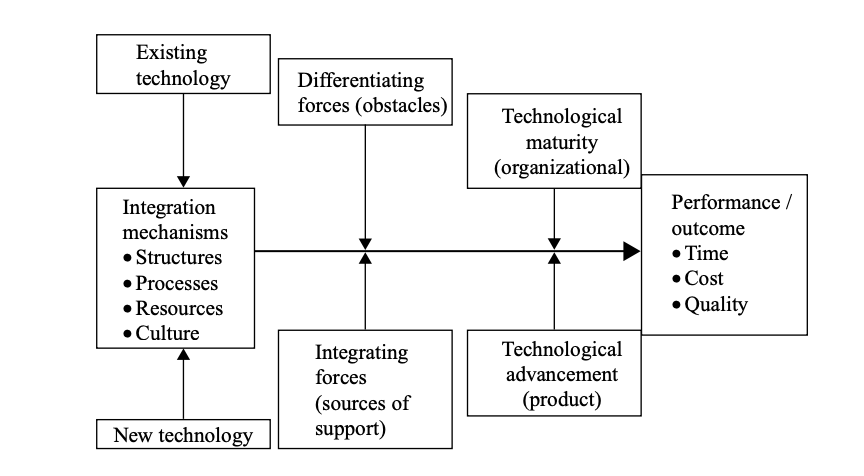
\includegraphics[width=0.8\textwidth]{Figure1.png}
    \caption{Conceptual model of the project change with implications and impact [1].}
    \label{fig:conceptual-model}
\end{figure}

\noindent The model in Figure 1 illustrates various things involved in during the project change and their impacts. Initially understanding the existing technology and the new to-be-adopted technology results in changes to the structures, processes, resources, and culture of the organization. Further into the picture are obstacles (differentiating forces) and sources of support (integrating forces) that influence the process. Finally, understanding the technological maturity of the current product/process and the advancement done to it, streamlining the analysis of their impacts, and taking deliberate steps based on this understanding as a project manager leads to favorable outcomes, benefiting the organization.

\subsection{Role of team experience in technology/process adoption}

The seamless adoption of technology within any project is intricately linked to the collaborative efforts of the involved team. The team's collective motivation, combined with their prior knowledge and skill sets, significantly shapes the trajectory of adoption, creating an environment conducive to successful integration. However, without proper attention, challenges such as resistance to change, gaps in knowledge, a resistant mindset, and a lack of collaboration can impede the technology/process adoption process. As rightly stated, "People's commitment to change increases the chance of successful transformation and decreases the cost of change. It is the most powerful catalyst for changing approach" [2].


\section{Methods \& Methodology}
In this section, we will explore methods and methodologies designed to address the challenges associated with technology adoption. Our focus will be on strategic steps that project managers can employ to ensure the successful adoption of technology. This encompasses effective approaches to mitigate resistance, enhance knowledge transfer, dealing with differentiating and integrating forces, fostering a positive mindset among the team, and promote collaborative practices that we learnt from above section. Additionally, we will delve into the critical aspect of analyzing costs and benefits related to the change adoption, securing buy-in, and implementing planning methods. 


\subsection{Analyzing costs and benefits}
\lipsum[20]

\subsection{Estimation Process}
\lipsum[15]

\subsection{Verification of Estimates}
\lipsum[16]

\subsection{Planning for change}
\lipsum[17]

\subsection{Securing Buy-In}
\lipsum[18]

\subsection{Overcoming Resistance}
\lipsum[19]


\section{Results Obtained}
\subsection{Under What Conditions}
\lipsum[21]

\subsection{Constraints}
\lipsum[22]

\subsection{Quality Assessment}
\lipsum[23]

\section{Conclusions and Future Works}
\subsection{Limitations to Solution}
\lipsum[24]

\subsection{Suggested Improvements}
\begin{itemize}
  \item \lipsum[25]
  \item \lipsum[26]
\end{itemize}

\subsection{Applications in Real World}
\lipsum[27]

\subsection{Conclusion}
\lipsum[28]

\section{References}
\begin{enumerate}
  \item Karlsson, C., Taylor, M., \& Taylor, A. (2010). Integrating new technology in established organizations: A mapping of integration mechanisms. \textit{International Journal of Operations \& Production Management, 30}(7), 672--699. Emerald Group Publishing Limited.
  
  \item Gandomani, T. J., Zulzalil, H., Ghani, A. A., Sultan, A. B. M., \& Sharif, K. Y. (2014). How human aspects impress Agile software development transition and adoption. \textit{International Journal of Software Engineering and Its Applications, 8}(1), 129--148.
\end{enumerate}

\section{Acknowledgements}
\lipsum[29]

\end{document}
